\chapter{Truncations for Stationary Distributions}\label{ch:statagg}
An important part of the analysis of such models concerns their long-run behavior.
Given an ergodic underlying Markov chain, the chain's stationary distribution characterizes this behavior.
For some special model classes, such as zero-deficiency networks~\parencite{anderson2011continuous}, analytical solutions for the stationary distribution are known.
However, most models require numerical approaches, often based on some form of approximation to guarantee tractability.
Those approaches can be based on stochastic simulation~\parencite{gillespie1977exact} (which for steady-state analysis tends to be slow and inaccurate) or moment-bounds via mathematical programming~\parencite{kuntz2017rigorous}.
Here, we draw on numerical approaches based on state-space truncation, which represent a viable option to approximate stationary distributions~\parencite{kuntz2021approximations}.
Truncation-based approaches have the benefit of describing the complete dynamics within a finite subset of the typically very large or infinite state-space.
As such, they enable the approximation of complex distributions that are not well-described by low-order moments.

%Luca: up to here.

The main step in the computation of such an approximation is the identification of a suitable truncation,
i.e.\ a subset of the state-space encompassing most of the stationary probability mass.
Existing methods typically rely on Foster-Lyapunov drift conditions to define such subsets~\parencite{dayar2011bounding}.
While these truncations come with bounds on the contained stationary probability mass, they typically are far larger than necessary.
The truncation is usually strongly constrained by the form of the chosen Lyapunov function~\parencite{gupta2014scalable,dayar2011bounding}.
Optimizing over possible functions to identify efficient truncations is technically challenging and, to our knowledge, has not been demonstrated for general reaction networks~\parencite{milias2014optimization}.

In this work, we address the identification of suitable truncations by using an aggregation-refinement scheme.
Initially, a Lyapunov analysis yields a set containing at least $1-\epsilon$ of the stationary probability mass.
On this subset of the state-space, we apply an aggregation scheme that groups together states in  hypercube macro-states.
Throughout each of these macro-states, we assume a uniform distribution among its constituent micro-states.
This allows us to roughly analyze large portions of the state-space with exponentially fewer variables.
We then iteratively truncate and refine the approximation based on the stationary distribution of this aggregated Markov chain. 
We keep only the most relevant macro-states and  continue this scheme until the macro-states contain a single original state. 
In this way, we arrive at an effective truncation to compute an approximation of the stationary distribution.

We investigate the approximation results on case studies with known stationary distributions and complex models with intricate stationary distributions.
We evaluate the truncation quality by assessing the stationary probability mass captured.
To this end, we use analytical solutions and bounds given by a Lyapunov analysis.
Further, we explore the control of the truncation size through the truncation parameter.
Finally, we demonstrate the method on the p53 oscillator model exhibiting a complex stationary distribution.


\section{Related Work}\label{sec:statagg:related}
\paragraph{Analytical Solutions}
For some specific models, analytical solutions for the stationary distribution have been found \parencite{melykuti2014equilibrium,kurasov2018stochastic}. For the class of zero-deficiency networks, the stationary distribution is known to have a Poisson product form \parencite{anderson2010product}. Monomol\-ecular reaction networks can be solved explicitly, as well~\parencite{jahnke2007solving}.

\paragraph{Truncation-Based Analysis}
The analysis of countably infinite-sized state-spaces is often handled by pre-defined truncations~\parencite{kwiatkowska2011prism}.
Sophisticated state-space truncations for the (uncon\-ditioned) forward analysis have been developed that give lower bounds.
They typically provide a trade-off between computational load and tightness of the bound~\parencite{munsky2006finite,lapin2011shave,andreychenko2011parameter,henzinger2009sliding,mikeev2013fly}.
Such methods cannot be directly applied to the estimation of stationary distributions because the approximation usually introduces a sink-state.

Truncations for stationary distributions often involve re-direc\-tion schemes for transitions leaving and entering the subset.
A comprehensive survey of such state-space truncation methods can be found in \parencite{kuntz2021stationary}.
A popular method of identifying truncations is the construction of a suitable Lyapunov function.
Beyond their use for establishing ergodicity \parencite{meyn1993stability,gupta2014scalable,dayar2011bounding},
these functions can be used to obtain truncations, guaranteed to contain a certain amount of stationary probability mass \parencite{dayar2011bounding}.
Using Lyapunov functions for the construction of truncations often leads to very conservative sets \parencite{milias2014optimization}.
Different approaches have been employed to find truncations:
In \citet{gupta2017finite} \ac{SSA} estimates are used to set up an increasing family of truncations.

\paragraph{Moment-Based Approximation}
Apart from approaches based on state-space truncations, moment-based approaches have been particularly popular recently~\parencite{ghusinga2017exact,dowdy2018bounds,kuntz2017rigorous,sakurai2017convex}.
Such approaches are based on the fact that particular matrices of distributional moments such as mean and variance are positive semi-definite.
Along with linear constraints stemming from the Kolmogorov equations \parencite{backenkohler2016generalized}, a semi-definite program can be formulated and solved using existing tools.
While this method is suited to compute bounds on both moments and subsets of the state-space, its application is limited, due to numerical issues inherent in the formulation \parencite{dowdy2018bounds}.

An approach where quantities are only described in terms of their magnitude has been proposed in \citet{ceska2019semi}. This allows for an efficient qualitative analysis of both dynamic and transient behavior.

\paragraph{Aggregation}
An aggregation scheme similar to the one used here has been previously proposed in \citet{backenkohler2020analysis} to analyze the bridging problem on Markov population models.
This is the problem of analyzing process dynamics under both initial and terminal constraints.

Aggregation-based numerical methods for computing the stationary distribution 
of discrete or continuous-time Markov chains have been studied in
previous work. Popular approaches rely on an alternation of aggregation and 
disaggregation of the state-space \parencite{stewart1994introduction,schweitzer1991survey}.
In the case of stiff chains, such aggregations are typically based on 
a separation of time-scales \parencite{cao1985iterative}.
However, these methods have been developed for finite chains with arbitrary structure and are motivated by numerical issues of standard methods such as 
the power method or Jacobi iteration \parencite{stewart1994introduction}.
They do not consider a truncation of irrelevant states, while
here our aggregation approach is used to determine the most relevant states
under stationary conditions in large or infinite chains with population structure.




%\section{Truncation-Based Approximation of $\pi_{\infty}$}\label{sec:statagg:fsp}
\section{Truncation-Based Approximation}\label{sec:statagg:fsp}
In many relevant cases, the state-space is huge or infinite and therefore the stationary solution cannot be computed directly.
To make such a computation possible we have to restrict ourselves to a finite manageable subset of the state-space and assume the majority of the probability mass is concentrated within that finite subset.
The main problem is to deal with the transitions leading to and from the truncated set (cf.\ \autoref{fig:truncation}).
In forward analysis, the outgoing transitions are simply redirected into a sink-state.
This way, a forward analysis provides lower bounds since mass leaving the truncation does not re-enter.
This approach, however, is unsuitable for the computation of stationary distributions because mass would accumulate in the sink-state leading to a distribution assigning all mass to it.
Therefore, transitions leaving the truncation need to be redirected back into the truncation.

The process' dynamics outside the truncation are defined by the \emph{stochastic complement} \parencite{spieler2014numerical}.
If its behavior was known, one could redirect outgoing to incoming transitions optimally and preserve the correct stationary distribution.
However, this reentry distribution is typically unknown in most relevant cases.
Many different reentry distributions have been used, such as redirecting to some internal state or states with incoming transition from outside the truncation.
\citet{kuntz2021approximations} provides a comprehensive review of such methods.

The most natural choice is to pick a reentry distribution that redirects mass to states with incoming transitions from truncated states (cf.\ \autoref{fig:truncation} (center)).

Using varying redirections, we can compute bounds on the stationary probability conditioned on a truncation \parencite[Thm.~14]{spieler2014numerical}.
To do this, one has to compute the stationary distribution for every possible way of connecting all outgoing to a single incoming transition.
Naturally, such an algorithm is rather expensive since one has to solve a linear system for each combination.
Therefore this method of computing bounds is costly on very large truncations, often given by Lyapunov functions.
In \autoref{fig:fsp_redirections} an enumeration of all such redirections is shown on a small $3\times 3$-truncation.
\begin{figure}[htb]
    \centering
    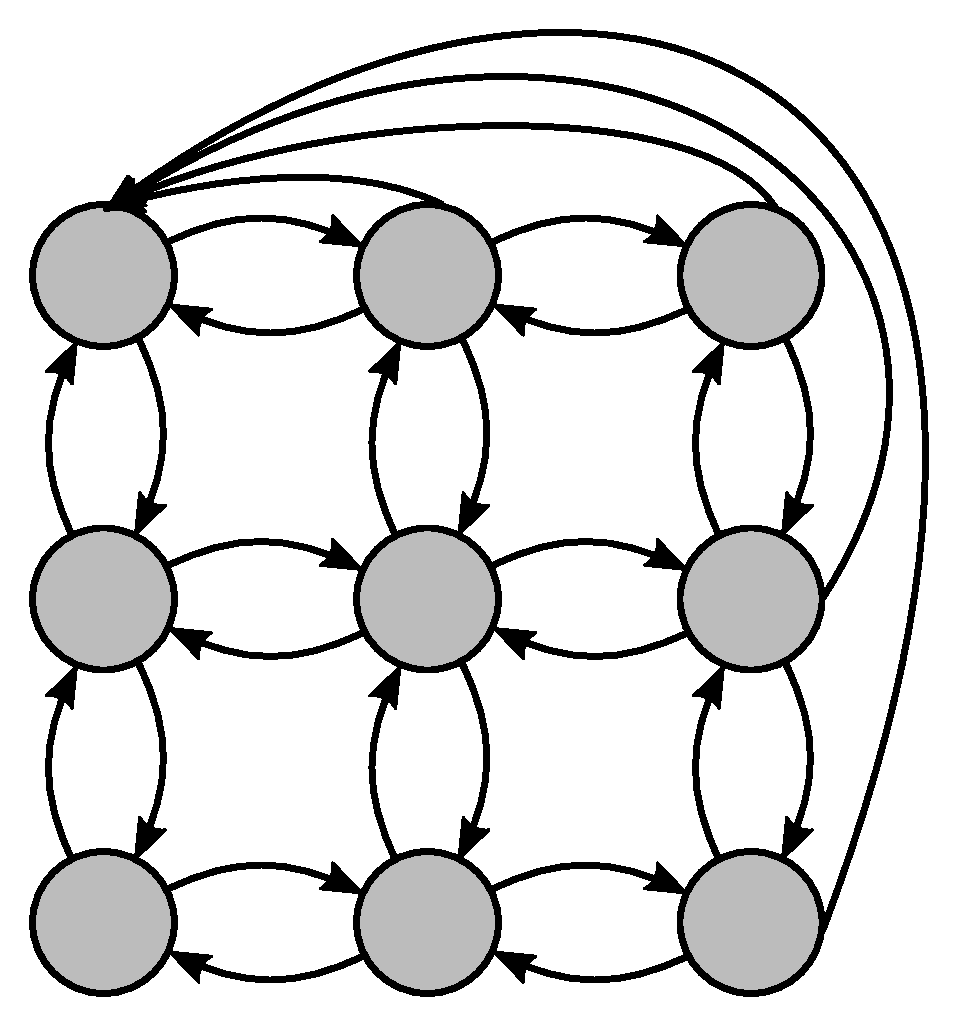
\includegraphics[width=0.19\textwidth]{gfx/state_space_redirected_1.pdf}
    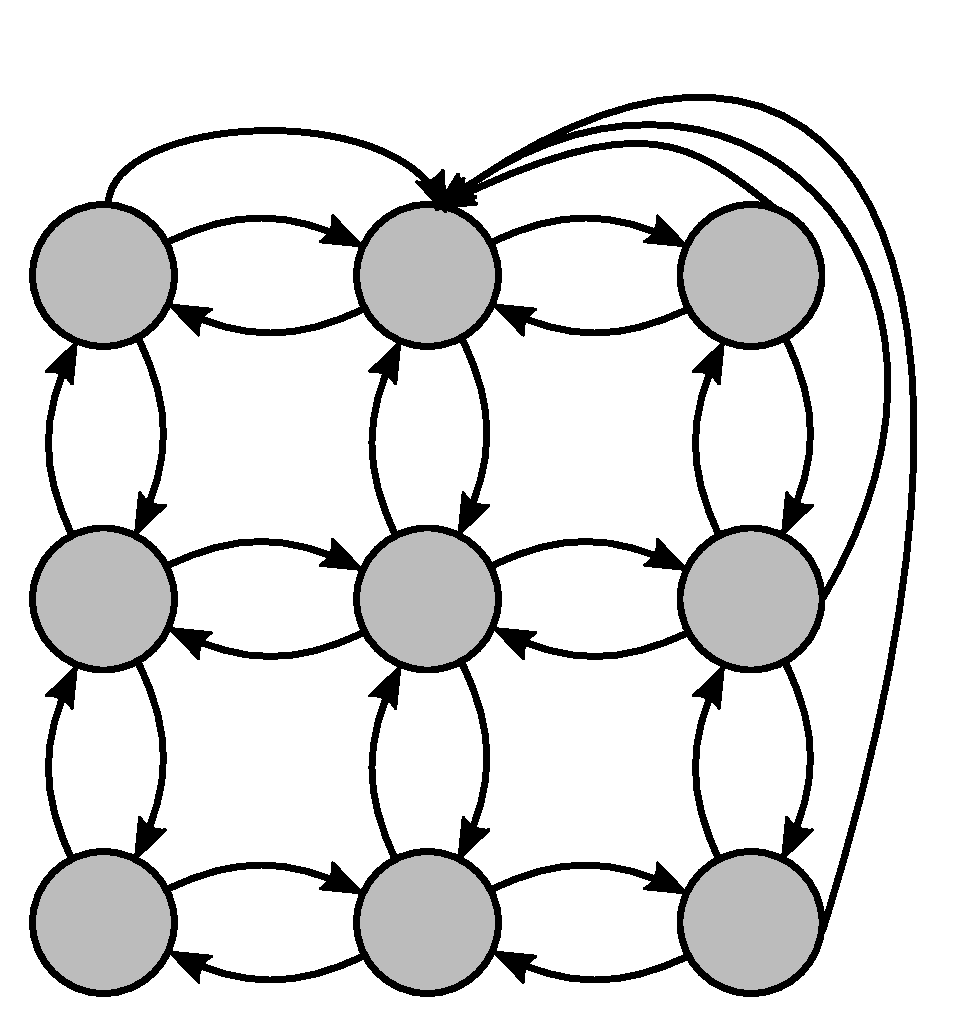
\includegraphics[width=0.19\textwidth]{gfx/state_space_redirected_2.pdf}
    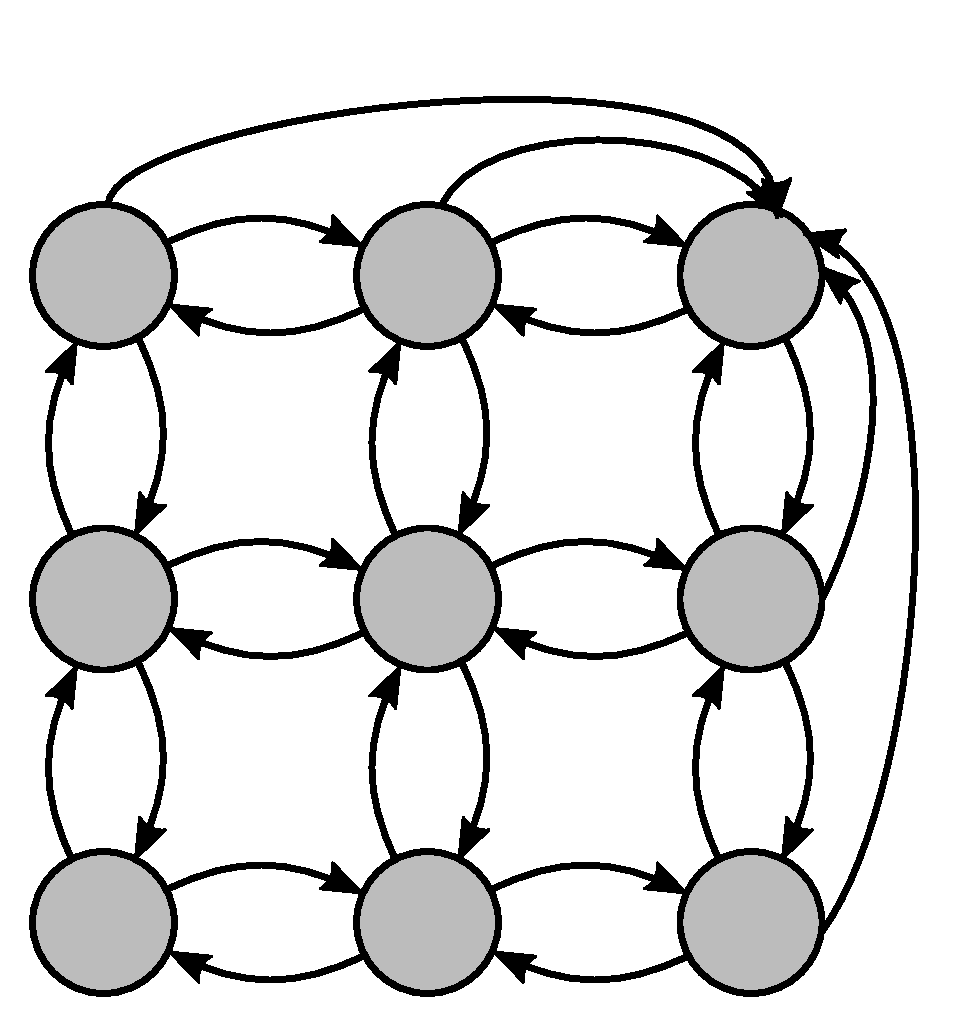
\includegraphics[width=0.19\textwidth]{gfx/state_space_redirected_3.pdf}
    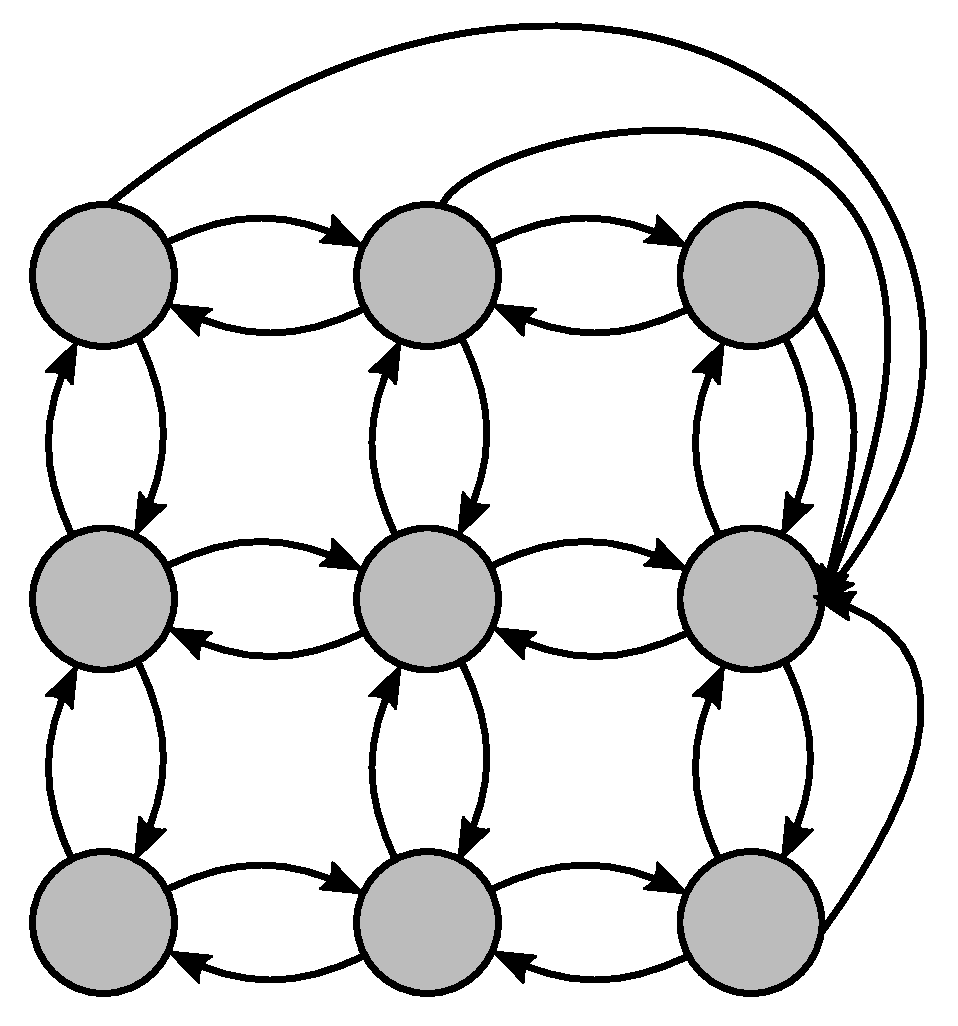
\includegraphics[width=0.19\textwidth]{gfx/state_space_redirected_4.pdf}
    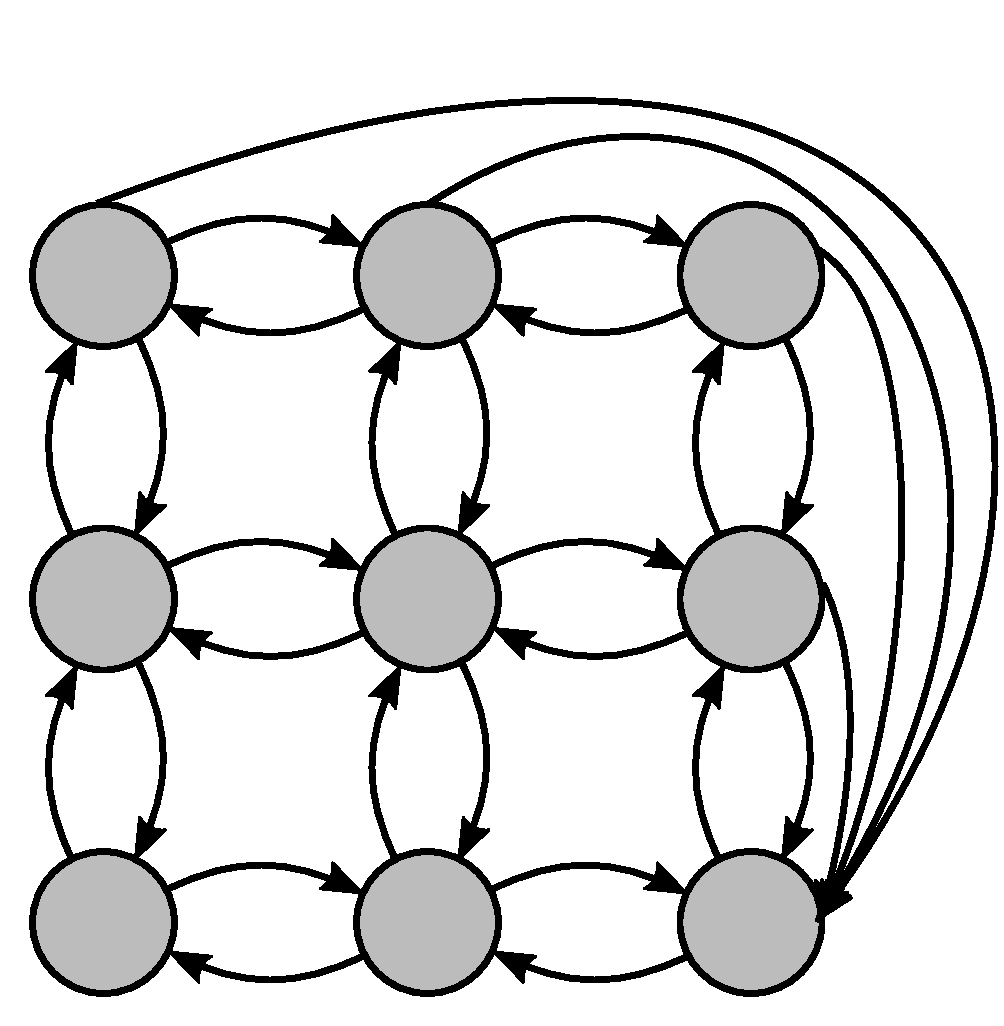
\includegraphics[width=0.19\textwidth]{gfx/state_space_redirected_5.pdf}
    \caption[Redirections for bounds]{Enumeration and solution of all single-state
    redirections yields upper and lower bounds on the stationary
    distribution, conditioned on being inside the truncation.\label{fig:fsp_redirections}}
\end{figure}

When computing an approximation instead of bounds, we employ a uniform redirection scheme:
Outgoing transitions are split uniformly among incoming transitions.
Due to the threshold-based truncation scheme, we are likely to end up with a somewhat uniform distribution over in-boundary states (see \autoref{sec:statagg:alg}).


The identification of good truncations remains a major task in such approximations.
Using approaches such as Lyapunov functions (\autoref{sec:statagg:lyapunov}) \parencite{dayar2011bounding} or moment-bounds \parencite{kuntz2021approximations} can provide a good initial estimate, but typically the resulting truncations are far larger than necessary.
This leads to dramatically increased computational costs, especially when bounding methods mentioned above are performed.
Until a system for a larger truncation is solved, the precise location of  most of the probability mass is often unknown.
Instead of solving the full system for such a large space, we employ an aggregation scheme to cover large areas of the state-space with exponentially fewer variables.

Error bounds have been derived for increasing  truncation sets 
in the case of linear Lyapunov functions  \parencite{gupta2017finite}.
However, until now it has not been shown that these bounds are applicable in practice \parencite{meyn1994computable}.
Alternatively, one can monitor the product of the probability-ouflow rate and the maximum L1-norm.
This bounds the approximation error up to a constant $M>0$, assuming a linear Lyapunov function exists \parencite{gupta2017finite}.


\begin{figure}[t]
    \centering
    \begin{minipage}{0.6\textwidth}
    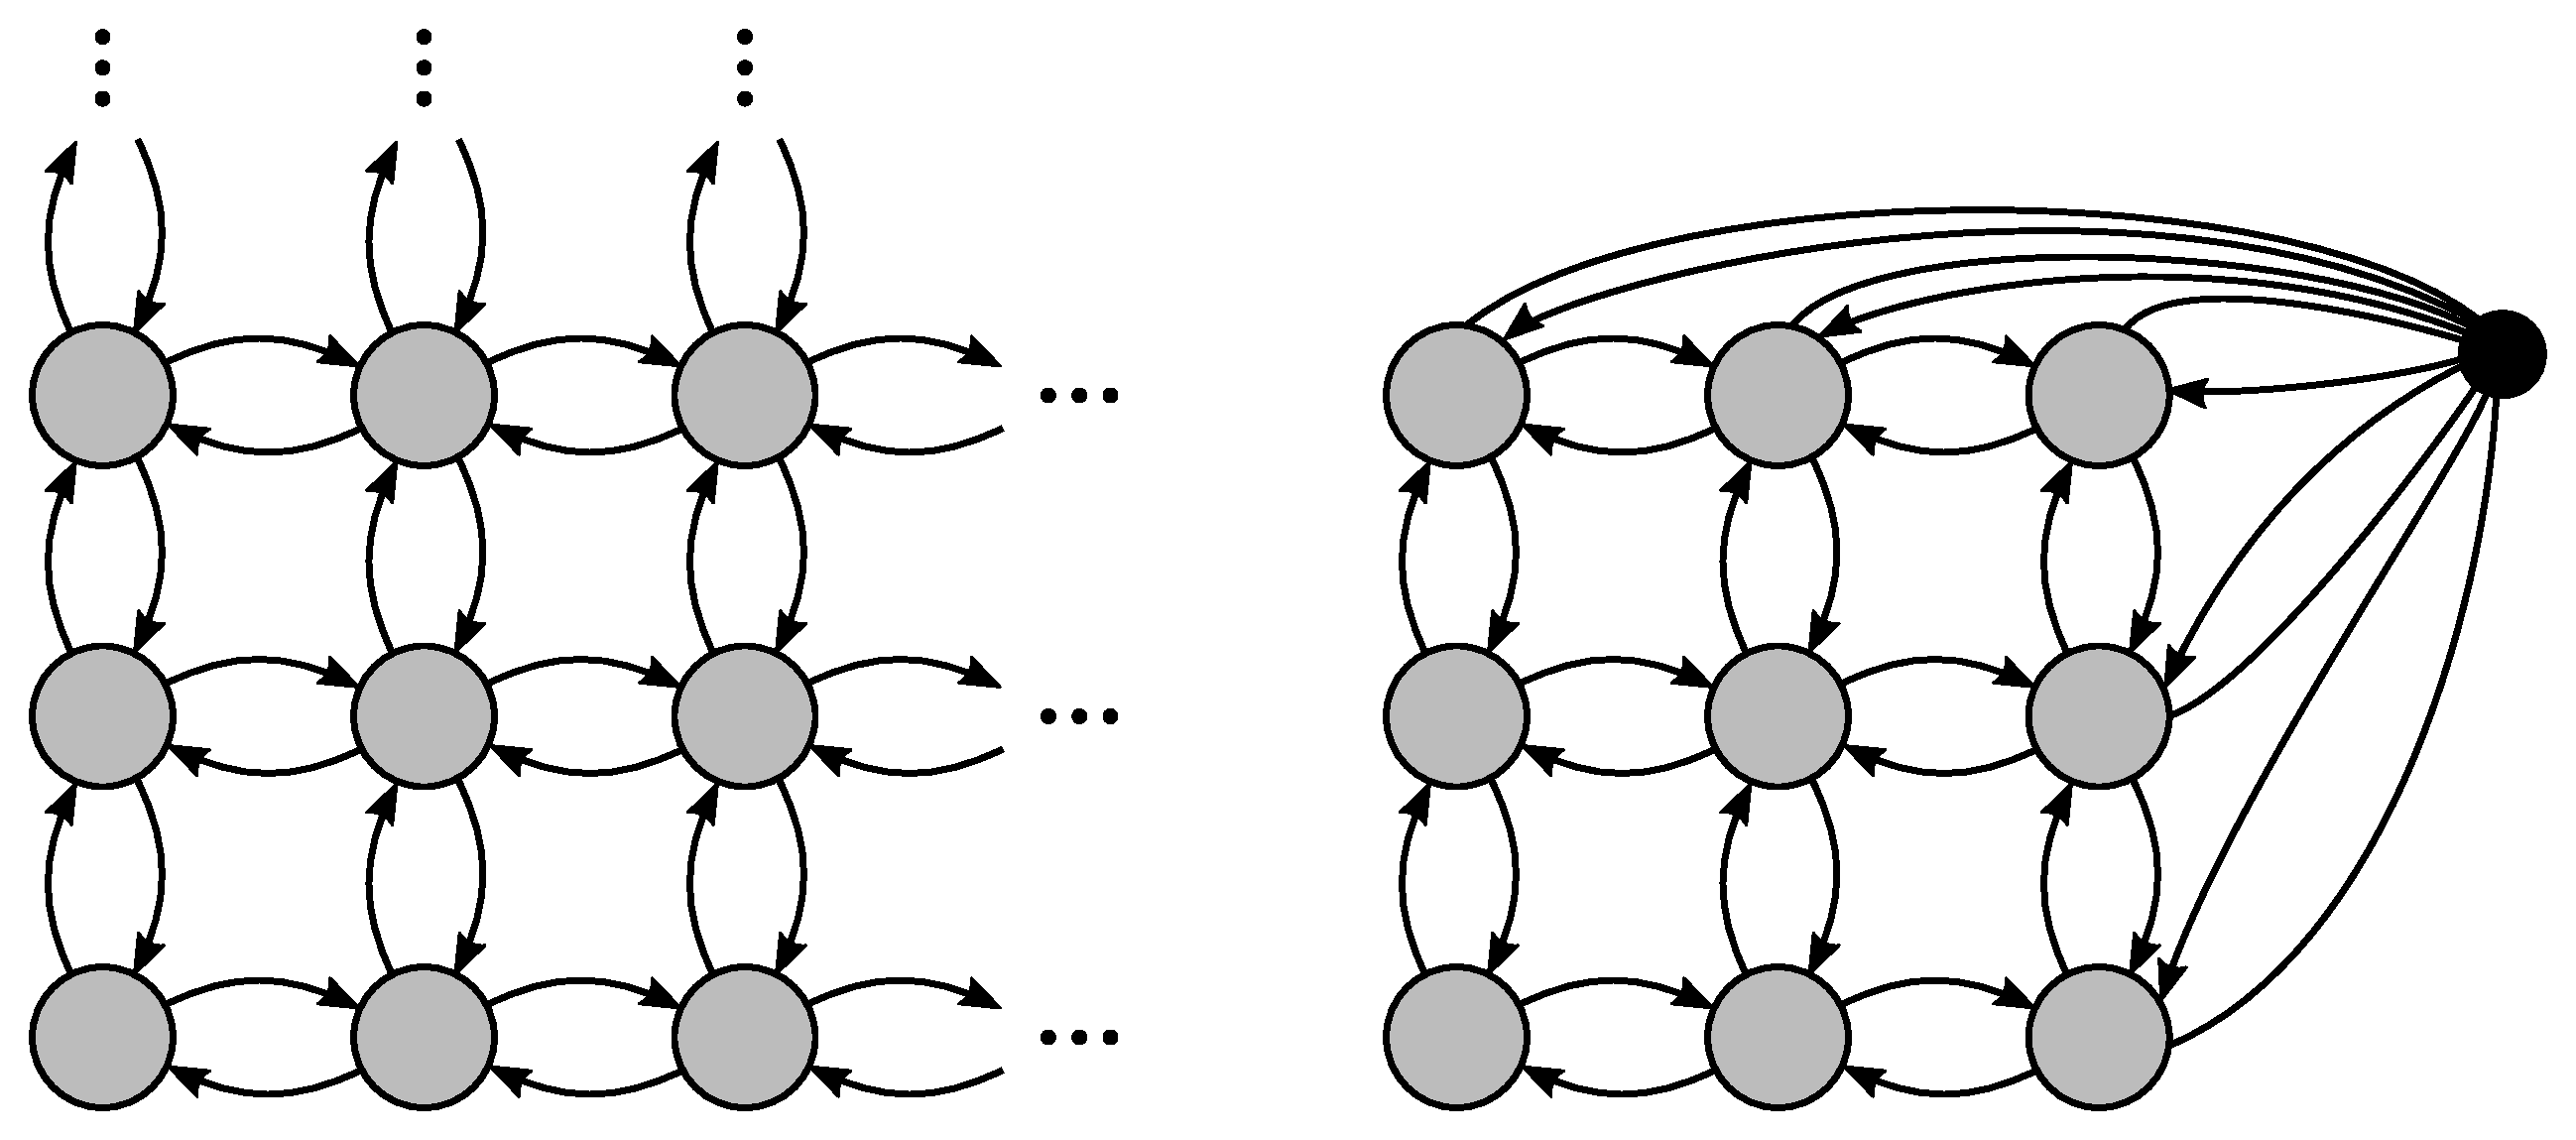
\includegraphics[width=\textwidth]{gfx/state_space_all.pdf}
    \end{minipage}
    \begin{minipage}{0.35\textwidth}
    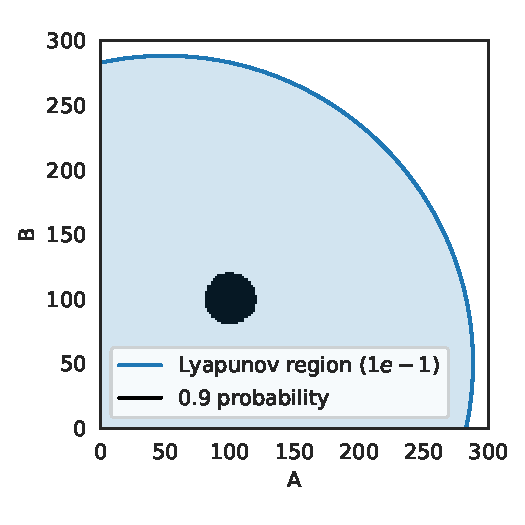
\includegraphics[width=\textwidth]{gfx/parbd_lya_v_truth.pdf}
    \end{minipage}
    \caption[Stationary \ac{FSP}]{(left) A countably infinite state-space. (center) Outgoing transitions are re-directed (according to the reentry distribution) to states that have incoming transitions from outside the truncation. (right) A comparison of the area prescribed by a Lyapunov analysis using Geobound and threshold \num{0.1} and the minimal area containing \num{0.9} stationary probability mass. The model is a parallel birth-death process (\autoref{model:par_bd}).}
    \label{fig:truncation}
\end{figure}




\subsection{Initial Aggregation}\label{sec:statagg:initagg}
The initial aggregated space $\hat{\mathcal{S}}^{(0)}$ should encompass all regions of the state-space that could contain significant mass because states outside this initial area will not be refined.
In principle, multiple approaches could be used to identify such a region.
One possibility is the computation of moment bounds for the stationary distribution~\parencite{ghusinga2017exact,dowdy2018bounds}.
Based on these bounds on expectations and covariances, an initial truncation could be fixed.
The approach we use here is to identify such a  region by a Lyapunov analysis \parencite{dayar2011bounding}.
This way, we obtain a polynomial describing a semi-algebraic subset of the entire state-space containing $1-\epsilon_{\ell}$ of the mass, where $\epsilon_{\ell}>0$ can be fixed arbitrarily.
These sets usually are far larger than a minimal set containing $1-\epsilon_{\ell}$ of stationary probability mass would be.
As an initial aggregation, we build an aggregation on a subset $[0..n]^{n_S}\subset \mathcal{S}$ containing the set prescribed by the Lyapunov analysis.
We also employ this approach to estimate errors in the evaluation.
Specifically, we employ the tool Geobound~\parencite{geobound} with L2-norm as function $g$ implementing techniques presented in \citet{dayar2011bounding}.

In many cases, simple choices of $g$ such as the L1- or L2- norm are sufficient.
However, the sets resulting from such functions are often very conservative.
Consider \autoref{fig:truncation} (right) as an example, where the Lyapunov truncation with $\epsilon_{\ell}=0.1$ %\vw{eps=0.1 sollte hier angegeben werden? }
for two parallel birth-death processes (\autoref{model:par_bd}) is compared to the smallest set containing \num{0.9} of stationary probability.
Clearly, the area given by the Lyapunov function is magnitudes larger than necessary to capture probability mass consistent with $\epsilon_{\ell}$.


\subsection{Iterative Refinement Algorithm}\label{sec:statagg:alg}
\begin{figure}[t]
    \centering
    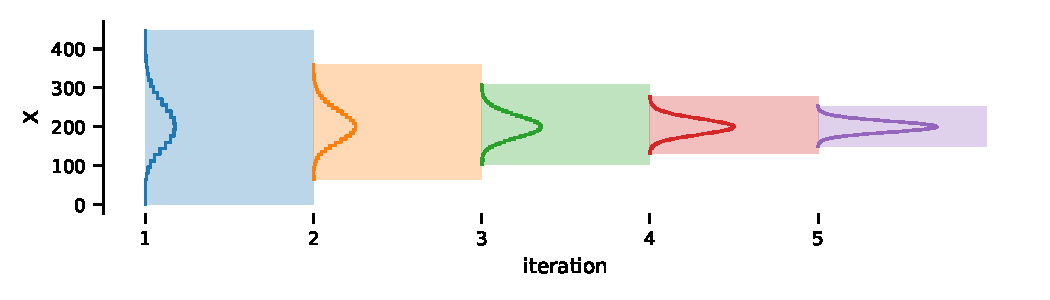
\includegraphics[width=\textwidth]{gfx/bd_truncs.pdf}
    \caption[State-space refinement algorithm]{The state-space refinement algorithm on a birth-death process. From left to right the state size is halved and states with low probability are removed from the truncation. The final truncation is a typical truncation with states of size 1 and the initial states are of size $2^4$.}
    \label{fig:refinement_alg}
\end{figure}


\begin{algorithm}
\SetKwFunction{Split}{split}
\SetKwInOut{Input}{input}
\SetKwInOut{Output}{output}
\Input{Initial partitioning $\mathcal{S}^{(0)}$, truncation threshold $\epsilon$}
\Output{approximate stationary distribution $\hat\pi_{\infty}$}
\For{$i=1,\dots,m$}{
    ${\hat\pi}^{(i)}_{\infty}\leftarrow $ approximate stationary distribution on $\mathcal{S}^{(i)}$\label{line:stationary}\;
    $\mathcal{R}\leftarrow$ smallest $\mathcal{R}'\subseteq\mathcal{S}^{(i)}$ s.~t. $ \sum_{\bar{x}\in\mathcal{R}'}\hat{\pi}_{\infty}^{(i)}(\bar{x})\geq1-\epsilon$\label{line:filter}\;
    $\mathcal{S}^{(i+1)}\leftarrow \bigcup_{\bar{x}\in\mathcal{R}} \text{split}(\bar{x})$\label{line:refine:stat}\;
    update $\hat{Q}$-matrix\label{line:update_q:stat}\;
}
\Return ${\hat\pi}^{(m)}_{\infty}$\;
    \caption{Approximating the stationary distribution }
    \label{alg:refinement:stat}
\end{algorithm}
The refinement algorithm (\autoref{alg:refinement:stat}) starts with a set of large macro-states
that are iteratively refined, based on approximate stationary distributions.
We start by constructing square macro-states of size
$2^m$ in each dimension for some $m\in\mathbb{N}$ such that they form a large-scale grid $\mathcal{S}^{(0)}$. 
Hence, each initial macro-state has a volume of ${\left(2^m\right)}^{n_S}$.
This choice of grid size is convenient because we can halve states
in each dimension.
Moreover, this choice ensures that all states have an equal volume
and we end up with unit-sized macro-states,
equivalent to a truncation of the original non-lumped state-space.

An iteration of the state-space refinement starts by computing the stationary distribution, using the lumped $\hat Q$-matrix.
Based on a threshold parameter $\epsilon>0$
states are either removed or split (\autoref{line:refine:stat}), depending on
the mass assigned to them by the approximate stationary
probabilities $\hat\pi^{(i)}_{\infty}$.
Thus, each macro-state is either split into $2^{n_S}$ new states or removed
entirely.
The result forms the next lumped state-space $\mathcal{S}^{(i+1)}$.
The $\hat{Q}$-matrix is updated (\autoref{line:update_q:stat}) using \eqref{eq:lumped_q} to calculate the transition rates of the next aggregated truncation $\mathcal{S}^{(i+1)}$. 
Entries of truncated states are removed from the updated transition matrix.
Transitions leading to them are
re-directed according to the re-entry matrix (\autoref{sec:statagg:fsp}).
After $m$ iterations (we started with states of side lengths $2^m$)
we have a standard \ac{FSP} scheme
on the original model tailored to
computing an approximation of the stationary distribution.


This way, the refinement algorithm focuses only on those parts of the state-space contributing most to the stationary distribution.
For instance, in \autoref{fig:refinement_alg} the stationary probability mass mostly concentrates around $\#S=200$.
Therefore, states that are further away from this area can be dropped in further refinement.
This filtering (\autoref{line:filter} in \autoref{alg:refinement:stat}) ensures that
states contributing significantly to $\hat\pi_{\infty}^{(i)}$ will be kept and refined in the next iteration.
The selection of states is done by sorting states in descending order according to their approximate probability mass.
This ensures the construction of the smallest possible subset chosen for refinement according to the approximation.
Then states are collected until their overall approximate mass is above $1-\epsilon$.

An interesting feature of   the aggregation scheme is that the distribution
tends to spread out more.
This is due to the assumption of a uniform distribution inside macro-states.
To gain an intuition, consider a macro-state that encompasses a peak of the stationary distribution.
If we re-distribute the actual probability mass inside this macro-state uniformly,
a higher probability is assigned to states at the macro-state's border.
When plugging such macro-states together, this increased mass away from the peak will
increase the mass assigned to adjacent macro-states.
This effect is illustrated by the example of a birth-death process in \autoref{fig:refinement_alg}.
Due to this effect, an iterative refinement typically keeps an over-approximation in terms of state-space area.
This is a desirable feature since relevant regions are less likely to be pruned due to lumping approximations.

\section{Results}\label{sec:statagg:results}
A prototype was implemented in Rust~1.50 and Python~3.8.
The linear systems were solved either using Numpy~\parencite{numpy} for up to \num{5000} states, or the sparse linear solver as available through Scipy~\parencite{2020SciPy-NMeth}, or the iterative biconjugate gradient stabilized algorithm~\parencite{van1992bi} (up to \num{10000} iterations and absolute tolerance \num{e-16}).

The examples that we consider in the sequel 
are typical benchmarks for the analysis of \acp{MPM}. For most of them, appropriate Lyapunov functions
have been determined using Geobound \parencite{geobound,spieler2014numerical}.
However, the corresponding Lyapunov sets containing at least $1-\epsilon_{\ell}$ of the stationary probability mass are very large for typical choices of $\epsilon_{\ell}$ (e.g. $\epsilon_{\ell}\in \{0.1,0.05,0.001\}$). Even
for extremely large $\epsilon_{\ell}$, say $\epsilon_{\ell}=0.8$, the remaining state-space may still be huge (e.g, \num{15198} states).
\subsection{Parallel Birth-Death Process}
We first examine the algorithm on the simple example of two parallel, uncoupled birth-death processes.
\begin{model}[Parallel Birth-Death Process]\label{model:par_bd}
Two uncoupled parallel birth-death processes result in a simple stationary distribution that is
given by a product of two Poisson distributions.
$$\varnothing\xrightarrow{\rho} A \qquad A\xrightarrow{\delta} \varnothing \qquad
\varnothing\xrightarrow{\rho} B \qquad B\xrightarrow{\delta} \varnothing$$
As a parameterization we choose $\rho = 100$ and $\delta=1$.
\end{model}
For this model, the stationary distribution is known to be the product of two Poisson distributions with rate $\rho / \delta$.

According to the Lyapunov analysis with a \e{1}{-4} bound, we fix the initial truncation to a $70\times 70$ grid of macro-states with size $2^7$ in each dimension.
This implies 8 iterations of the algorithm to arrive at a truncation with the original granularity.
In \autoref{fig:par_bd}, we illustrate the truncations of different iterations.
Over the iterations, the covered area decreases, while the aggregation granularity increases.
The final truncation distribution approximation is also depicted and covers $1 - \e{1.27}{-2}$ of the true stationary distribution (cf.\ \autoref{tab:intervals:par_bd}).

For this case study, we also compute state-wise bounds on the probabilities conditioned on the truncation as discussed in \autoref{sec:statagg:fsp}.
In \autoref{fig:par_bd_errors}, we present the difference between upper and lower bound for $\epsilon=0.1$.
We observe intervals that are narrowest in the truncation's interior near the distribution's mode.
The largest intervals or the largest absolute uncertainty is present in the boundary states.
This indicates, that the specific reentry distribution has little effect on the main approximate stationary mass.
More detailed results on the intervals' magnitudes are given in \autoref{tab:intervals:par_bd}.
\begin{figure}[htb]
    \centering
    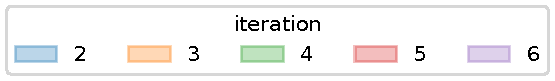
\includegraphics[scale=0.7]{gfx/iteration_legend.pdf}\\
    \vspace{-5mm}
    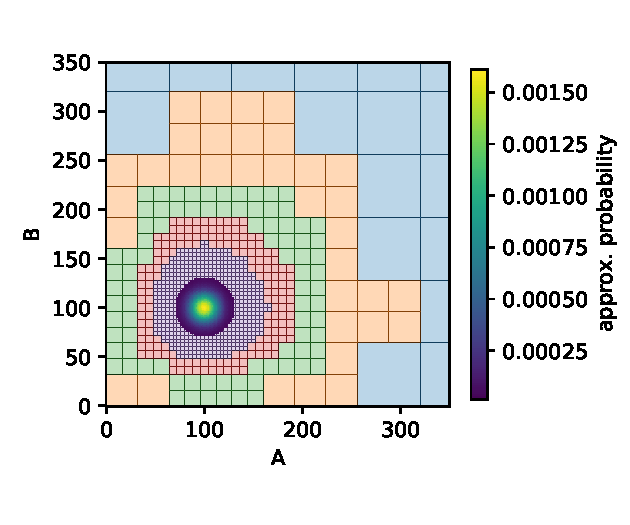
\includegraphics[width=.75\textwidth]{gfx/parbd_truncs.pdf}
	\caption[Overview of truncation refinements]{\label{fig:par_bd}Truncations of different iterations are layered on top of each other. At higher iterations, truncations cover less area but increase in detail, due to the refinement of macro-states. The final approximation is indicated by its approximate probabilities.}
\end{figure}
\begin{figure}[htb]
	\centering
    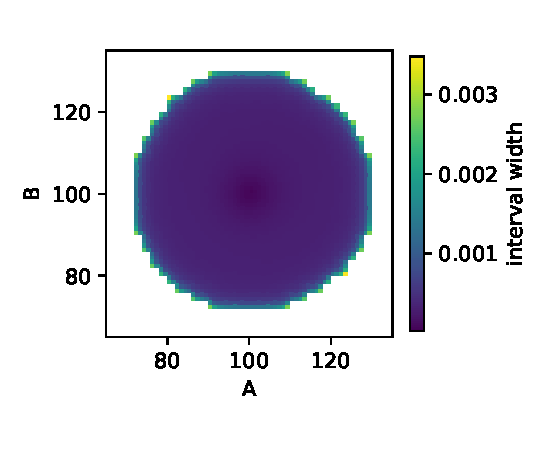
\includegraphics[width=.6\textwidth]{gfx/diffs.pdf}
	\caption[Probability bound widths]{Results for \autoref{model:par_bd} with truncation threshold $\epsilon=0.1$.  The difference between the upper and lower bounds on the probability conditioned on the truncation.}
    \label{fig:par_bd_errors}
\end{figure}
\begin{figure}
    \centering
    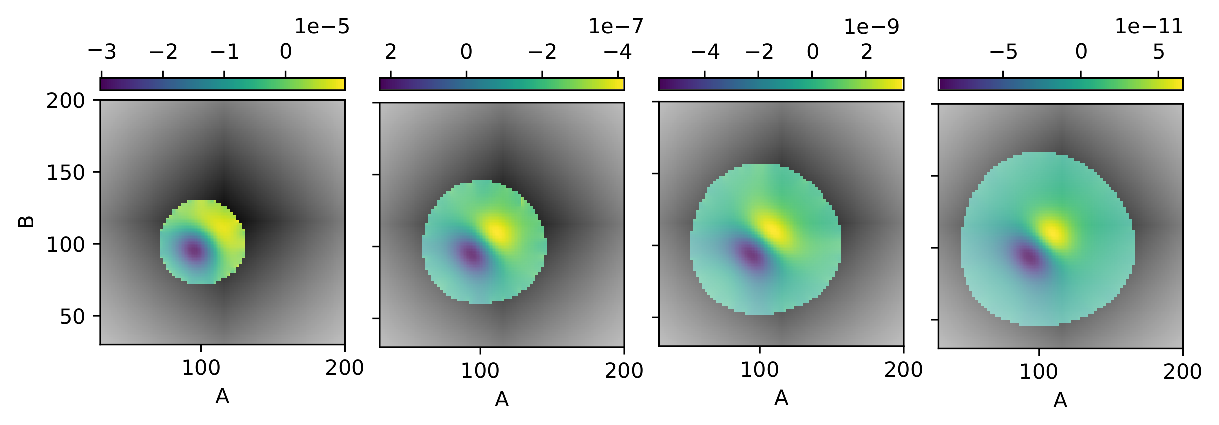
\includegraphics[width=\textwidth]{gfx/par_bd_errs.eps}
    \caption[Stationary distribution errors]{\label{fig:par_bd_errs}Errors of the stationary distribution (\autoref{model:par_bd}) approximations for increasing ($\e{1}{-1}$, $\e{1}{-2}$, $\e{1}{-3}$, $\e{1}{-4}$) truncation thresholds.}
\end{figure}
\begin{table}
    \centering
	{\small \begin{tabular}{lrrrr}% L{22mm} R{15mm} R{15mm} R{15mm} R{15mm}}
    \toprule
      & \multicolumn{4}{c}{threshold parameter $\epsilon$} \\\cmidrule(lr){2-5}
	    & \e{1}{-1} & \e{1}{-2} & \e{1}{-3} & \e{1}{-4} \\
     \midrule
	    total width & $1.2336$ & \e{3.09}{-2} & \e{5.39}{-4} & \e{8.12}{-6} \\
	    max.\ width &  \e{3.47}{-3} & \e{9.29}{-5} & \e{4.04}{-7} & \e{4.65}{-9} \\
	    outside mass & \e{1.27}{-2} & \e{1.05}{-4} & \e{1.05}{-6} & \e{1.06}{-8} \\
         \bottomrule
	\end{tabular}}
	\caption[Probability bound properties for approximation of the stationary distribution]{Results for \autoref{model:par_bd} : The characteristics of the lower-upper bound intervals on the conditional probability and the mass not contained in the truncation are given.}
    \label{tab:intervals:par_bd}
\end{table}
% \begin{figure}
%     \centering
%     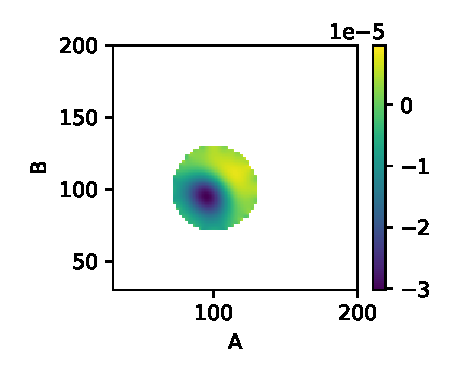
\includegraphics[width=0.48\textwidth]{gfx/par_bd_errs_0.1.pdf}
%     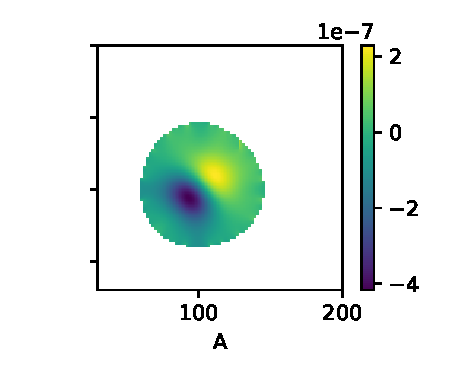
\includegraphics[width=0.48\textwidth]{gfx/par_bd_errs_0.01.pdf}
%     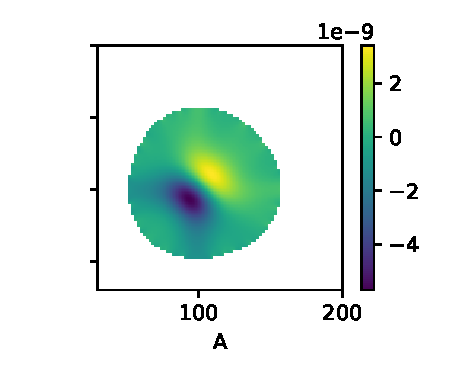
\includegraphics[width=0.48\textwidth]{gfx/par_bd_errs_0.001.pdf}
%     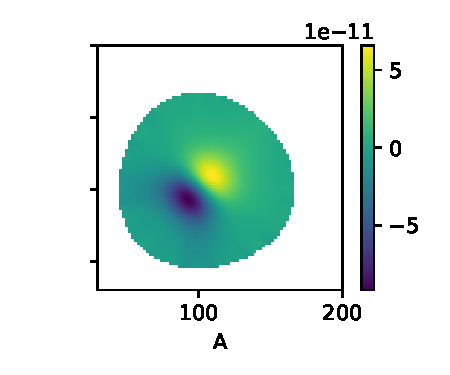
\includegraphics[width=0.48\textwidth]{gfx/par_bd_errs_0.0001.pdf}
%     \caption{The error over the truncation wrt.\ the analytical solution}
% \end{figure}

\subsection{Exclusive Switch}
The exclusive switch~\parencite{barzel2008calculation}  has three different modes of operation, depending on the
\ac{DNA} state, i.e.\ on whether a protein of type one or two is bound to
the \ac{DNA}.

\begin{model}[Exclusive Switch]\label{model:excl_switch}
The exclusive switch model consists of a promoter region
that can express both proteins $P_1$ and $P_2$. Both can bind to the region, suppressing
the expression of the other protein. For certain parameterizations, this leads to a
bi-modal or even tri-modal behavior.
$$ D \xrightarrow{\rho_1} D + P_1 \qquad D \xrightarrow{\rho_2} D + P_2 \qquad P_1 \xrightarrow{\lambda}\varnothing \qquad P_2 \xrightarrow{\lambda} \varnothing $$
$$ D + P_1 \xrightarrow{\beta} D.P_1 \qquad D.P_1 \xrightarrow{\gamma_1} D + P_1 \qquad D.P_1 \xrightarrow{\rho_1} D.P_1 + P_1 $$
$$ D + P_2 \xrightarrow{\beta} D.P_2 \qquad D.P_2 \xrightarrow{\gamma_2} D + P_2 \qquad D.P_2 \xrightarrow{\rho_2} D.P_2 + P_2 $$
We choose parameter values $\rho_1 = 0.7$, $\rho_2 = 0.6$, $\lambda=0.02$, $\beta=0.005$, $\gamma_1 = 0.06$, and $\gamma_2 = 0.05$.
\end{model}
Since the exclusive switch models mutually exclusive binding of proteins to a single genetic locus,
we know a priori that there are exactly three distinct operating modes.
In particular are $D$, $D.P_1$, and $D.P_2$ mutually exclusive such that \[X_{D}(t) + X_{D.P_1}(t) + X_{D.P_2}(t) = 1, \quad \forall t\geq 0\,.\]
This model characteristic often leads to bi-modal stationary distributions, where one or the other protein is more abundant depending on the genetic state.

Accordingly, we adjust
the initial truncation:
The state-space for the \ac{DNA} states is not lumped. Instead we ``stack''
lumped approximations of the $P_1$-$P_2$ plane upon each other.
Such special treatment of \ac{DNA} states is common for such models \parencite{lapin2011shave}.
Using Lyapunov analysis for threshold $0.001$, we fix an initial state-space of $63\times 63$ macro-states with size $2^7$. Detailed results for different parameters $\epsilon$ are presented \autoref{tab:excl_switch}\turnto{tab:excl_switch}.
We compute error bounds using a worst-case analysis based on reference solutions provided by Geobound with $\epsilon_{\ell}=0.01$.
We observe a strong decrease in both upper bounds on the total absolute and maximal absolute error in the final iteration.
Interestingly, the errors between different thresholds are very close in earlier iterations.
This is mainly due to the usage of absolute errors which causes probabilities close to the mode dominate.
\begin{figure}[htb]
    \centering
    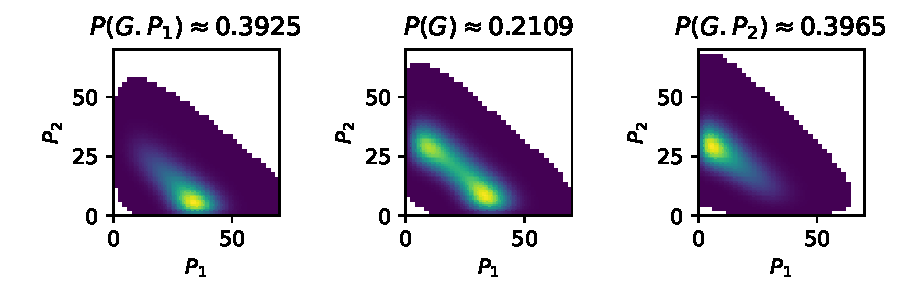
\includegraphics[width=\textwidth]{gfx/gexpr_approx.pdf}
	\caption[Approximate stationary distribution of the exclusive switch]{The approximate stationary distribution of the exclusive switch (\autoref{model:excl_switch}) obtained with $\epsilon=\e{1}{-4}$.}
    \label{fig:excl_switch:excl_switch_dist}
\end{figure}


Using Geobound we observe that our final truncation captures the stationary mass very well (cf.\ \autoref{tab:intervals} and \autoref{fig:excl_switch:excl_switch_dist}).
We use the Geobound's lower bounds with $\epsilon_{\ell}=\e{1}{-2}$ and find that the uncovered mass by the aggregation-based truncation is magnitudes lower than $\epsilon$ or close to it (for $\epsilon=0.1$).
While they capture the mass well, they are much smaller than the Geobound truncation ($\epsilon_{\ell}=0.1$) % \vw{?} 
with \num{16780} states, regardless of the threshold parameter $\epsilon$.
\begin{table}[htb]
    \centering
	{\small \begin{tabular}{lrrrr}%{L{30mm} R{14mm} R{14mm} R{14mm} R{14mm}}
    \toprule
      & \multicolumn{4}{c}{threshold parameter $\epsilon$} \\\cmidrule(lr){2-5}
	    & \e{1}{-1} & \e{1}{-2} & \e{1}{-3} & \e{1}{-4} \\
     \midrule
	    total width & $5.5171$ & $1.5559$ & \e{2.89}{-2} & \e{3.71}{-4} \\
	    max.\ width & \e{1.58}{-1} & \e{3.30}{-3} & \e{3.47}{-5} & \e{3.84}{-7} \\
	    outside mass $\leq$ & \e{1.52}{-1} & \e{1.29}{-3} & \e{2.02}{-5} & \e{2.72}{-7} \\
         \bottomrule
    \end{tabular}
	}
	\caption[Characteristics of the lower-upper bound intervals]{Results for \autoref{model:excl_switch}: The characteristics of the lower-upper bound intervals on the conditional probability and the upper bound on mass not contained in the truncation are given.}
    \label{tab:intervals}
\end{table}

In \autoref{fig:excl_switch:trunc_sizes}, we show the effect of the threshold parameter $\epsilon$ on the size of the final truncation.
We observe a roughly linear increase in size with an exponential decrease of $\epsilon$.
\begin{figure}[htb]
    \centering
    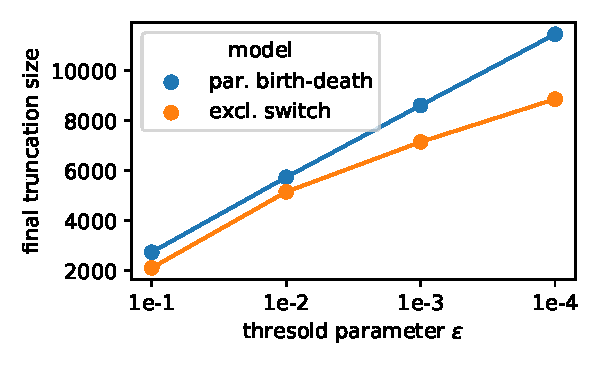
\includegraphics[scale=.7]{gfx/trunc_sizes.pdf}
	\caption[The sizes of the final truncation v.\ the threshold parameter $\epsilon$]{The sizes of the final truncation vs.\ the threshold parameter $\epsilon$ (\autoref{model:bd} and \autoref{model:excl_switch}).}
    \label{fig:excl_switch:trunc_sizes}
\end{figure}

\subsection{p53 Oscillator}
We now consider a model of the interactions of the tumor suppressor p53~\parencite{geva2006oscillations}. The system describes the negative feedback loop between  p53 and the oncogene Mdm2.
Species pMdm2 models a precursor to Mdm2. This model is particularly interesting due to its complex three-di\-mea\-nsional oscillatory behavior.
The model is ergodic with a unique stationary distribution~\parencite{gupta2014scalable}.
\begin{figure}[htb]
    \centering
    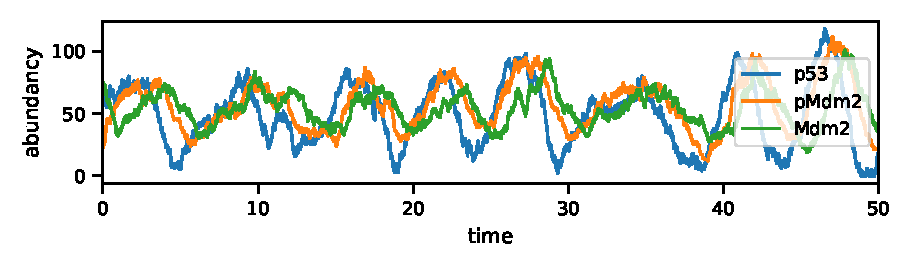
\includegraphics[width=\textwidth]{gfx/p53_traj.pdf}
    \caption{A sample trajectory illustrating the oscillatory long-run behavior. }
    \label{fig:p53:traj}
\end{figure}
\begin{model}[p53 Oscillator]\label{model:p53}
\begin{align*}
\varnothing \xrightarrow{k_1} \mathrm{p53} \qquad
\mathrm{p53} \xrightarrow{k_2} \varnothing \qquad
\mathrm{p53} \xrightarrow{k_4} \mathrm{p53} + \mathrm{pMdm2}
\\
\mathrm{p53} \xrightarrow{\alpha_4(\cdot)} \varnothing \qquad
\mathrm{pMdm2} \xrightarrow{k_5} \mathrm{Mdm2} \qquad
\mathrm{Mdm2} \xrightarrow{k_6} \varnothing
\end{align*}
The non-polynomial degradation reaction rate
	\[
\alpha_4(x) =k_3 x_{\mathrm{Mdm2}} \frac{x_{\mathrm{p53}}}{x_{\mathrm{p53}} + k_7}\,.
\]
The parameterization based on \parencite{ale2013general} is $k_1=90$, $k_2=0.002$, $k_3=1.7$, $k_4=1.1$, $k_5=0.93$, $k_6=0.96$, and $k_7 = 0.01$.
\end{model}
With the exception of propensity function $\alpha_4$, we can compute the transition rates ${\bar{\alpha}}_i$ using the Faulhaber formulae, as discussed in \autoref{ch:lumping}.
We consider $\alpha_4$ separately, because it is non-polynomial and therefore, we have to make an approximation.
The fraction occurring in the non-linear propensity function $\alpha_4$ can roughly be characterized as an activation function:
Due to the low value of parameter $k_7=0.01$ we can approximate\graffito{Note, that $\sum_{i=0}^n i / (i + k_7)$ can be solved analytically. However, the approximation presented above is much simpler to compute.}
\[\frac{x_{\mathrm{p53}}}{x_{\mathrm{p53}} + k_7}
\approx
\begin{cases}
0 & \text{if } x_{\mathrm{p53}} = 0\\
1 & \text{otherwise}
\end{cases}
\]
We use this approximation at the coarser levels of aggregation to efficiently compute the approximate transition rate $\bar{\alpha}_4$.
At the finest granularity we switch back to exact propensity function $\alpha_4$.

We now derive Lyapunov-sets for the p53 oscillator case study (Model~\ref{model:p53}). Let the Lyapunov function
\begin{equation}
    g(x) = 120 x_{\mathrm{p53}} + 0.2 x_{\mathrm{pMdm2}} + 0.1 x_{\mathrm{Mdm2}}\,.
\end{equation}
Then the drift
\begin{equation}\label{eq:p53_drift}
\begin{split}
    d(x) = & - \frac{k_3 x_{\mathrm{Mdm2}} x_{\mathrm{p53}}}{x_{\mathrm{p53}} + k_7}
            - 0.1 k_6 x_{\mathrm{Mdm2}}
            + 120 k_1 \\
          & - 120 k_2 x_{\mathrm{p53}}
            + 0.2 k_4 x_{\mathrm{p53}}
            - 0.1 k_5 x_{\mathrm{pMdm2}}  \\
        = & - \frac{204 x_{\mathrm{Mdm2}} x_{\mathrm{p53}}}{x_{\mathrm{p53}} + 0.01}
            - 0.096 x_{\mathrm{Mdm2}}
            - 0.02 x_{\mathrm{p53}} \\
            &- 0.0093 x_{\mathrm{pMdm2}}
	    + \num{10800}\,. 
\end{split}
\end{equation}
Clearly, $c = \sup_{x\in{S}} d(x) = \num{10800}$.
In particular, the supremum $c$ is at the origin since all non-constant terms are negative.
The slowest rate of decrease for \eqref{eq:p53_drift} is $x_{\mathrm{p53}}$ with $x_{\mathrm{Mdm2}} = x_{\mathrm{pMdm2}} = 0$.
We are content with a superset of a Lyapunov set \eqref{eq:lyapunov_set} for some threshold $\epsilon_{\ell}$.
Therefore taking \eqref{eq:lyapunov_set}, we can solve the inequality
\[
	\frac{\epsilon_{\ell}}{c}(c - \num{0.02} x_{\mathrm{p53}}) > \epsilon_{\ell} - 1
\]
for $x_{\mathrm{p53}}$ and 
\begin{equation*}
    \frac{c}{0.02 \epsilon_{\ell}} < x_{\mathrm{p53}}\,.
\end{equation*}
Therefore
\begin{equation*}
\pi_{\infty}\left(\left\{x\in\mathcal{S} \mid \frac{c}{0.2\epsilon_{\ell}} < \lVert x \rVert \right\}\right) > 1 - \epsilon_{\ell}\,.
\end{equation*}

Due to the exponential increase stemming from the three-di\-men\-sion\-al nature of this model, we only evaluated with parameter $\epsilon=0.1$.
According to the Lyapunov analysis shown above, the area covered by an $6\times 6\times 6$ macro-states with size $2^{20}$, covers \num{0.9} of stationary mass.
A truncation of this same area would consist of \num{226492416} states instead of the \num{216} macro-states.
The model has a striking oscillatory behavior (cf.\ \autoref{fig:p53:traj}) that is reflected in its stationary distribution.
This feature is well-captured in the approximate distribution, where the oscillatory behavior leads to a complex stationary distribution (cf.\ \autoref{fig:p53:dist}).
This distribution leads to a non-trivial truncation (\num{357488} states) which is tailored to the main stationary mass (\autoref{fig:p53:trunc}).
\begin{figure}[htb]
    \centering
    \begin{minipage}{0.9\textwidth}
    \centering
    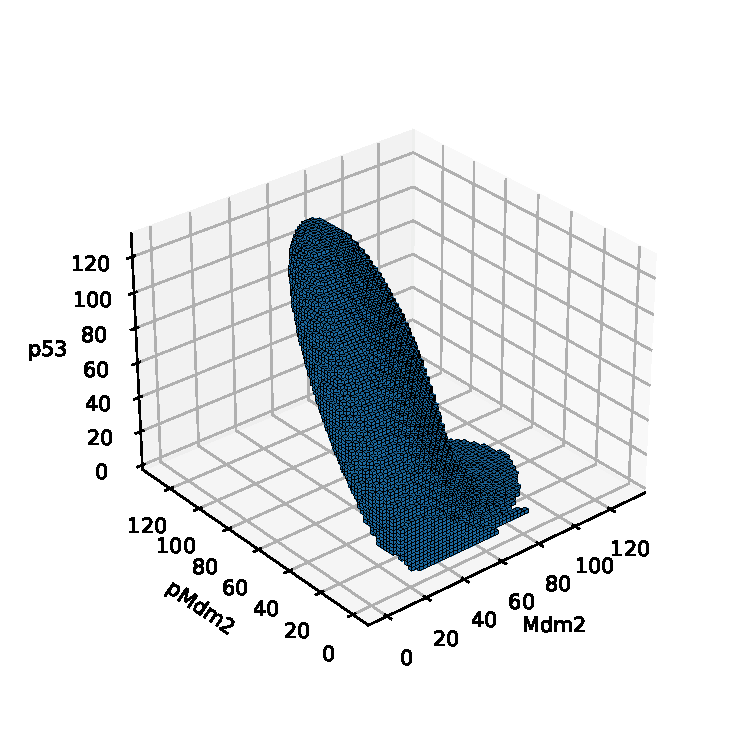
\includegraphics[width=\textwidth]{gfx/trunc_p53.pdf}
    \end{minipage}
\caption{The final truncation at original granularity derived for the p53 oscillator.}
\label{fig:p53:trunc}
\end{figure}
\begin{figure}[htb]
    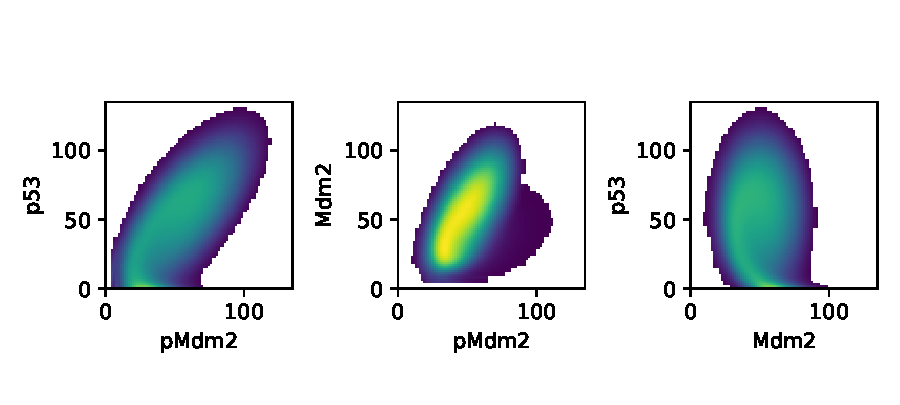
\includegraphics[width=.9\textwidth]{gfx/p53_dist.pdf}
	\caption[approximate marginal distributions of the p53 stationary distribution]{The approximate marginal distributions of the stationary distribution based on the truncation derived with $\epsilon=0.1$.}
\label{fig:p53:dist}
\end{figure}

\section{Conclusion}
State-of-the-art methods for numerically calculating the stationary distribution of \aclp{MPM} rely on coarse truncations of irrelevant parts of large or infinite discrete state-spaces. 
These truncations are either obtained from the stationary statistical moments of the process or from
Lyapunov theory. They are limited in shape because these methods do not take into account the detailed 
steady-state flow within the truncated state-space but only consider the average drift or stationary moments.

Here, we propose a method to find a tight truncation
that is not limited in its shape and iteratively optimizes the set based on numerically cheap solutions
of abstract intermediate models. 
It   captures the main portion of probability mass even in the case of complex behaviors efficiently.
In particular, the method represents another option, where Lyapunov analysis leads to forbiddingly large truncations.


